\documentclass[12pt]{report}
\usepackage{mathpartir}
\usepackage{amsmath}
\usepackage{amssymb}
\usepackage{multicol}
\usepackage[utf8x]{inputenc}
\usepackage[french]{babel}
\usepackage{graphicx}

\title{Typage d'un lambda-calcul avec une construction de branchements}
\author{Frédéric Bour, avec l'encadrement de Yann Régis-Gianas}

\newcommand\todo[1]{TODO[#1]}
\includeonly{langage}

\begin{document}

\maketitle

%%%%%%%%%%%%%%%%%%%%%%%%%%%%%%%%%%%%%%%%%%%%%%%%%%%%%%%%%%%%%%%%%%%%%%%%%%%%%%%%
%%%%%%%%%%%%%%%%%%%%%%%%%%%%%%%%%%%%%%%%%%%%%%%%%%%%%%%%%%%%%%%%%%%%%%%%%%%%%%%%

\chapter{Motivations}

Ce TRE a débuté par une étude de la faisabilité d'une analyse statique du
flot des exceptions pour OCaml 4.00. 

Les systèmes d'exceptions permettent au programmeur de manipuler le contrôle de
flot beaucoup plus librement qu'avec un traditionnel appel de fonction
retournant une valeur. Malheureusement, il devient alors difficile de connaître
les différents flots d'exécutions possibles car ceux-ci ne correspondent plus
strictement à la structure du code source -- on parle de contrôle de flot
non-local.

Les programmes sûrs issus d'OCaml font partie des principaux arguments en sa
faveur. Mais pour garantir cette sûreté, il faut souvent se priver
d'exceptions.  L'analyse statique que nous souhaitions effectuer visait à
vérifier de manière mécanique l'absence d'exceptions ou bien l'exhaustivité de
leur traitement dans un code source.

Ce travail reprenait les résultats de la thèse de François Pessaux
\cite{ExcAnalysis} qui avait abouti à un prototype permettant ce type d'analyse
pour OCaml 3.00.  Les résultats étaient très encourageants au point de
présenter un intérêt immédiat pour des applications industrielles.

Malheureusement, ce prototype n'a pas été porté vers les versions suivantes
d'OCaml et nous sommes arrivé à la conclusion que ce travail était trop
conséquent pour s'inscrire dans le cadre d'un TRE.  De plus, si l'approche
abordée dans la thèse permet une analyse fine, l'implantation est difficile à
maintenir car celle-ci s'appuie sur la syntaxe abstraite d'OCaml et implique de
développer en parallèle un typeur spécialisé.

Notre travail de recherche s'est alors orienté vers le langage intermédiaire du
compilateur OCaml. 

\section{\emph{Lambda}, le langage intermédiaire}

Cibler \emph{Lambda} apporte de nombreux avantages, notamment :
\begin{description}
  \item[Indépendance vis-à-vis du \emph{front-end}.] Si le langage de surface
    OCaml est régulièrement étendu, \emph{Lambda} est très stable et n'a pas
    connu de changements majeurs depuis l'introduction du système objet il y a
    plus de 10 ans. C'est une cible pérenne.(\todo{ref OO})
  \item[Langage minimaliste.]
    Les nombreuses constructions de surface sont réduites à un petit ensemble.
		La définition de \emph{lambda} tient en une dizaine de lignes ;
		la définition du langage de surface en occupe des centaines.
    L'analyse peut ainsi se concentrer directement sur le cœur du langage et
    garder une taille modeste. Le travail de maintenance est moindre.
\end{description}

Mais \emph{lambda} n'est pas typé. Dans la chaîne de traitement du
compilateur, les types sont vérifiés pour le langage source par le typeur puis
effacés. Tout le reste du traitement s'effectue sur une version non-typée du
programme. Ce choix est justifié par l'omniprésence du polymorphisme
paramétrique dans ce langage et de la représentation très régulière des valeurs
à l'exécution.

Le polymorphisme paramétrique permet de garantir qu'un programme bien typé est
sémantiquement équivalent après effacement des types \todo{ref didier rémy ?}.
La représentation des valeurs permet de travailler correctement sans
information de types -- cela concerne par exemple la convention d'appel des
fonctions ou le passage du glaneur de cellule.

\todo{figure : pipeline ocaml}.

Ce choix restreint les traitements possibles dans la suite de la compilation.
Le compilateur natif tente par exemple de réinférer des types dans le cadre de
certaines optimisations, mais il ne s'agit que d'approximation conservative.
Dans notre cas analyser le flot devient beaucoup plus compliqué -- un travail
absurde quand on sait que les informations nécessaires pour guider cette
analyse viennent d'être effacées dans la chaîne de compilation.

Concevoir une version de \emph{lambda} préservant les types semble être un
prérequis pour un outil d'analyse viable.

\section{Vers une version \emph{typée} de \emph{Lambda}}

Le langage \emph{lambda} est un lambda-calcul proposant des fonctions de très
bas-niveau.

Dans le cadre de la compilation, le lambda-calcul désigne une famille de
langage de programmation fonctionnelle reposant autour d'un unique mécanisme
d'abstraction.  Cela rend sa définition simplissime, le noyau syntaxique tient
en trois règles.  Mais derrière celles-ci se cache une très grande expressivité
: c'est un langage turing-complet et d'un suffisamment haut-niveau pour
permettre un encodage léger des constructions classiques des langages de
programmation \cite{LTU}.

Un lambda-calcul est ainsi un choix naturel pour un langage intermédiaire. La
variante d'OCaml ajoute principalement des primitives d'accès mémoires et de
branchements; des extensions de bas-niveau.

Une autre implantation majeure du langage de programmation fonctionnelle
Haskell, GHC \cite{Marlow98thenew}, a fait un choix très différent dans la
conception de son langage intermédiaire nommé \emph{Core}
\cite{Sulzmann07systemf}.  Ce dernier est typé et n'offre pas de telles
primitives; les accès mémoires sont masqués derrière une forme simplifiée de
\emph{filtrage de motifs}. Ce design
influencera nos choix par la suite.

\section{Le typage des constructions de bas-niveau}

Les systèmes de types d'OCaml et d'Haskell présentent de nombreuses
similitudes. La réussite de \emph{Core} nous a conforté dans la faisabilité
d'un traitement similaire pour OCaml.

Dans le souci d'être le moins intrusif possible dans le compilateur
OCaml actuel, il était nécessaire d'étendre le langage \emph{lambda} et non de
le remplacer.

Pour mener à terme cet objectif, les étapes suivantes se profilaient :
\begin{itemize}
  \item concevoir un système de type s'inspirant de System $F_c$ et composant
    avec les contraintes imposées par \emph{lambda},
  \item établir encodage des constructions d'Ocaml (types algébriques, modules,
    GADTs, variants polymorphes) dans ce système afin de s'assurer que toutes
    sont capturées,
  \item étendre \emph{lambda} et proposer un schéma de compilation vers ce
    nouveau langage intermédiaire.
\end{itemize}

Ceci constitue un travail de grande ampleur. Dans ce rapport nous adressons le
point précis de typer les contraintes imposées par \emph{lambda}; un
branchement et des accès mémoires beaucoup plus libres que ce que ne permet le
\emph{filtrage de motif} traditionnel.



%%%%%%%%%%%%%%%%%%%%%%%%%%%%%%%%%%%%%%%%%%%%%%%%%%%%%%%%%%%%%%%%%%%%%%%%%%%%%%%%
%%%%%%%%%%%%%%%%%%%%%%%%%%%%%%%%%%%%%%%%%%%%%%%%%%%%%%%%%%%%%%%%%%%%%%%%%%%%%%%%

\chapter{Solutions étudiées}

Tout n'est pas nécessaire, points principaux :

\section{Échec du typage structurel}

\subsection{Succès du typage nominal}

- encodage des exceptions
- encodage des GADTs
- encodage des variants
  - traduction du langage ML
    shift, extraction de tags, …

%%%%%%%%%%%%%%%%%%%%%%%%%%%%%%%%%%%%%%%%%%%%%%%%%%%%%%%%%%%%%%%%%%%%%%%%%%%%%%%%
%%%%%%%%%%%%%%%%%%%%%%%%%%%%%%%%%%%%%%%%%%%%%%%%%%%%%%%%%%%%%%%%%%%%%%%%%%%%%%%%

\chapter{Conception d'un langage approprié}

Le langage développé reprend le cœur du lambda-calcul polymorphe (Système F)
et l'étend avec les notions de primitives et de \emph{bloc} munie d'un
\emph{tag} et les constructions d'analyse de tag et d'aiguillage.

Présentons tout d'abord le noyau de ce langage.

\section{Lambda-calcul polymorphe} 

Les trois premières constructions du langage sont les variables, l'application
et l'abstraction. Elles forment lambda-calcul simplement typé.

Ces trois constructions permettent de construire et d'appliquer des fonctions,
dont le type est noté par une \emph{flèche} paramétré par le domaine et le
codomaine de la fonction.

L'application et l'abstraction de types rajoutent le polymorphisme, représentée
au niveau des types par la quantification universelle.

Contrairement à un langage tel qu'OCaml, la généralisation et l'instantiation
des valeurs polymorphes sont marquées explicitement. Si un tel langage devait
être utilisé dans le compilateur, c'est lors de la traduction que celles-ci
seraient ajoutées par le \emph{frontend}.

\section{Représentation des valeurs d'OCaml}

Les extensions ont été conçues autour de la représentation des valeurs par
OCaml. Les valeurs concrètes sont :
\begin{itemize}
  \item soit des entiers, directement représenté par un scalaire,
  \item soit des blocs représentés par un pointeur vers une
zone mémoire composée d'un \emph{tag} et d'un vecteur de valeurs.
\end{itemize}
Un bit des valeurs est réservé pour distinguer les entiers des pointeurs.

\todo{introduire les notions de types algébriques, variants … ?}
\paragraph{Types algébriques} Les constructeurs constants sont encodés par des
entiers, les constructeurs paramétrés par un bloc de même arité.

Les valeurs des entiers et les tags des blocs servent à discriminer les
différents constructeurs durant le \emph{filtrage de motif}. Les entiers
endossent ainsi le même rôle que le \emph{tag} du bloc.
 
\paragraph{Variants polymorphes} L'encodage ressemble à celui des types
algébriques, mais le \emph{tag} pour discriminer les constructeurs paramétrés
n'est plus celui du bloc. Une indirection est ajoutée sous la forme d'un
premier bloc composé du \emph{tag} et d'un pointeur vers le n-uplet contenant
les paramètres.

Le \emph{tag} devient ici une valeur de première classe, manipulable dans le
langage.  En particulier, celui-ci peut-être testé et transformé par
l'application d'opérateurs.

\begin{figure}
\centering
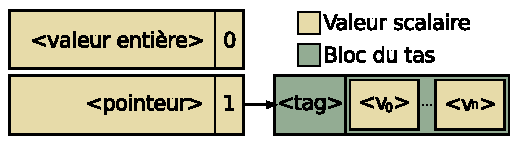
\includegraphics{media/ocaml_value}
\caption{Forme des valeurs}
\end{figure}

\begin{figure}
\centering
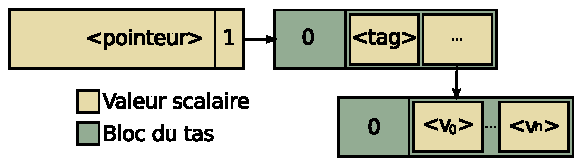
\includegraphics{media/ocaml_variant}
\caption{Forme des variants polymorphes}
\end{figure}

\section{Séparer extraction et analyse d'un \emph{tag}}

La principale contribution réside entre la séparation du calcul d'un tag et du
branchement qui s'ensuivra.

\paragraph{Filtrage de motif} Traditionnellement dans les langages ML, le
\emph{filtrage de motif} est utilisé pour permettre de manière sûre et efficace
la sélection de différentes branches de code.

Les constructeurs d'un type algébrique deviennent chacun une branche. Dans
chaque branche, des noms liés aux paramètres du constructeur testé sont
introduits. Le programmeur n'indique jamais explicitement l'accès aux champs
d'une valeur. Il ne peut même pas nommer un champ en dehors de la branche.

Il est alors simple de vérifier l'exhaustivité du traitement et de garantir
l'absence d'accès à des valeurs inexistantes lors de l'exécution. Enfin le
compilateur se voit offrir beaucoup de libertés pour générer du code efficace
\todo{cite Lefessant, Maranget, … compilation pattern matching}.

\paragraph{Motifs compilés} Le compilateur OCaml choisit de compiler ces motifs
très tôt. Dans le langage \emph{Lambda} il n'existe déjà plus que deux formes
de tests, les \emph{switch} et \emph{if} que l'on retrouve dans les langages
impératifs classiques. Une forme spécialisée de branchement proche du
\emph{goto} est aussi proposée pour factoriser le code des branches.

Les filtrages de haut-niveau sont ainsi traduits via des arbres de décisions,
au travers d'une suite de tests et de tables de sauts.  Le lien entre la
sélection d'une branche et les hypothèses qui y ont amené disparaît -- le
compilateur ne peut que suivre les instructions de projection sous l'hypothèse
que le code traduit est correct.


%%%%%%%%%%%%%%%%%%%%%%%%%%%%%%%%%%%%%%%%%%%%%%%%%%%%%%%%%%%%%%%%%%%%%%%%%%%%%%%%
%%%%%%%%%%%%%%%%%%%%%%%%%%%%%%%%%%%%%%%%%%%%%%%%%%%%%%%%%%%%%%%%%%%%%%%%%%%%%%%%

% Metavars
\newcommand\term{t}
\newcommand\ty{\tau}
\newcommand\tyenv{\Gamma}
\newcommand\csenv{C}

% Term
\newcommand\var{x}
\newcommand\app[2]{#1\,#2}
\newcommand\lam[2]{\lambda #1. #2}

% Value
\newcommand\val{v}

% Type
\newcommand\tyconst{\iota}
\newcommand\tyvar{\alpha}
\newcommand\tykind{*}
\newcommand\tyarrow[2]{#1 \rightarrow #2}
% Datatype
\newcommand\dtype{\epsilon \, \vec{\ty}}

% Binding
\newcommand\binding[2]{(#1 : #2)}

% Typing environment
\newcommand\tyenvnil{\bullet}
\newcommand\tyenvcons[3]{#1; \binding{#2}{#3}}

% Jugements
\newcommand\tycheck[3]{#1 \vdash #2 : #3}
\newcommand\tyenvmem[2]{#1 \in #2}

% Keyword
\newcommand\kw[1]{\operatorname{#1}}

% Pattern
\newcommand\pator{\;|\;}

% Operation semantic
\newcommand\redto[2]{#1 \longrightarrow #2}

% Naming rules
\newcommand\rname[1]{\;\;\textsc{{\small(#1)}}}
\newcommand\rref[1]{\textsc{\small#1}}
\newcommand\rcase[1]{\paragraph{Cas \rref{#1}:}}

\newcommand\freeinenv[1]{#1 \# \tyenv}
\newtheorem{thm}{Théorème}
\newtheorem{lemma}{Lemme}

\section{Formalisation du langage}

Le langage développé reprend le cœur du lambda-calcul polymorphe
\cite{Reynolds94anintroduction} (aussi connu sous le nom de \emph{Système F})
et l'étend avec les notions de primitives et de \emph{bloc} muni d'un
\emph{tag} et les constructions d'analyse de tag et d'aiguillage.

\subsection{Syntaxe}

Présentons tout d'abord la syntaxe de ce langage.

\subsubsection{Lambda-calcul polymorphe} 

Les trois premières constructions du langage sont les variables, l'application
et l'abstraction. Elles forment le lambda-calcul simplement typé.

$$\synp{\term_1, \term_2} \var, y$$
%
Référence à une variable (liée dans l'environnement).

$$\synp{\term_1, \term_2}   \term_1 \, \term_2$$
%
Application d'un terme à un autre.

$$\synp{\term_1, \term_2}   \lambda \binding{\var}{\ty} . \term$$
%
Abstraction par rapport à une variable; $\var$ est liée dans $\term$.

Ces trois constructions permettent de construire et d'appliquer des fonctions,
dont le type est noté par une \emph{flèche} paramétrée par le domaine et le
codomaine de la fonction.

L'application et l'abstraction de types rajoutent le polymorphisme, représenté
au niveau des types par la quantification universelle.

$$\synp{\term_1, \term_2}   \lambda \tyvar . \term$$
%
Cette construction lie $\tyvar$ au sein du terme $\term$.

$$\synp{\term_1, \term_2}   \term \, \ty $$
%
Contrairement à un langage tel qu'OCaml, la généralisation et l'instanciation
des valeurs polymorphes sont marquées explicitement. Si un tel langage devait
être utilisé dans le compilateur, c'est lors de la traduction que celles-ci
seraient ajoutées par le \emph{front-end}.

\subsubsection{Primitives}

Des primitives peuvent être appliquées via la construction :
%
$$\synp{\term_1, \term_2} prim \, \vec{\term}$$

Leur comportement est proche de celui de fonctions, mais elles ne sont pas
définissables dans le langage. Leurs règles de réduction et de typage seront
explicitées après.

Les primitives sont toujours invoquées avec tous leurs arguments (il n'y a pas
d'applications partielles).

\begin{description}
  \item[$\kw{makeblock}_{n,\dtype}$] Allocation d'un bloc avec l'étiquette $n$
    et le type $\dtype$.
  \item[$\kw{field}_n$] Projection du n-ième champ d'un bloc.
  \item[$\kw{eq}_z$] Test d'égalité avec la constante $z$.
  \item[$\kw{lt}_z$] Test d'infériorité par rapport à la constante $z$.
  \item[$\kw{isint}$] Test si une valeur est une constante ou un bloc.
  \item[$\kw{isout}_{[z1,z2]}$] Test si une valeur entière est dans un
    intervalle.
\end{description}

\subsubsection{Extraction d'étiquette} 

$$\synp{\term_1, \term_2} \kw{unpack} \term_1 \kw{as} y : \var \kw{in} \term_2$$
%
$\var$ et $y$ sont liés dans $\term_2$ :
\begin{itemize}
  \item $y$ est lié à la valeur de l'étiquette de $\term_1$.
  \item $\var$ devient un alias de $\term_1$, mais dont le type est raffiné en
    fonction des tests effectués sur $y$.
\end{itemize}

\subsubsection{Aiguillage} 

$$\synp{\term_1, \term_2} \kw{switch} \term \kw{in} \vec{b} : \ty$$
%
L'étiquette de $\term$ est testée contre les branches de $\vec{b}$.
L'exécution se poursuit sur la branche qui satisfait le test.

Les branches ont les formes suivantes :
%
$$\synp{b} n \rightarrow \term \; | \; b$$
%
Le test réussit si l'étiquette est égale à $n$.
%
$$\synp{b}  \_ \rightarrow \term$$
%
Cas par défaut, le test réussit toujours.
%
$$\synp{b} \emptyset$$
%
Tous les cas ont été couverts. Si l'exécution devait arriver sur ce cas, ce
serait une erreur. En particulier, le système de type doit garantir que ce cas
ne peut arriver à l'exécution.

\subsubsection{Constructeurs de types}

Soit $\epsilon$ l'ensemble des noms des constructeurs de types.
Sur cet ensemble sont définis les opérations suivantes:
\begin{description}
  \item[$ar(\epsilon)$] Associe à un nom de type le nombre de paramètres dont il
    dépend.
  \item[$dom(\dtype)$] Retourne l'ensemble des étiquettes que peuvent posséder
    les termes de types $\dtype$.
  \item[$Phi(\dtype, k, \var)$] Associe à une instance d'un type
    l'ensemble des contraintes à introduire dans l'environnement si l'on
    découvre que la variable $\var : \dtype$ a l'étiquette $k$.
  \item[$fields(\dtype,k)$] Retourne le vecteur des types des paramètres des
    valeurs du type $\dtype$ ayant l'étiquette $k$. Si le vecteur est vide,
     il n'y a qu'une seule valeur de ce type avec cette étiquette,
     c'est l'entier $k$.
\end{description}

On suppose de plus l'existence d'un type nommé \emph{int} dont les valeurs sont
les entiers naturels.

Enfin, pour chaque type de l'utilisateur on construit un ensemble de types
dérivés de la définition de ce type. Les éléments de cet ensemble sont décrits
dans la section \ref{metaconstr}.

\subsubsection{Algèbre de type}

$$\synp{\ty_1, \ty_2} \tyvar, \beta$$
%
Référence à des variables de types.

$$\synp{\ty_1, \ty_2}  \ty_1 \rightarrow \ty_2$$
%
Type d'une fonction de $\ty_1$ vers $\ty_2$.

$$\synp{\ty_1, \ty_2}  \forall \tyvar. \ty$$
%
Type polymorphe, abstrait par rapport à $\tyvar$ qui est lié dans $\ty$.

$$\synp{\ty_1, \ty_2}  \dtype$$
%
$\epsilon$ est un nom de constructeur de type, dont les paramètres sont
instanciés avec les types de $\vec{\ty}$.

$$\synp{\ty_1, \ty_2}  \{ \var \}_{\dtype}$$
%
Type singleton : c'est le type exact de la variable nommée $\var$. Celui-ci est
affiné par les contraintes introduites dans l'environnement.

$$\synp{\ty_1, \ty_2}  \{ n: \vec{\ty} \}$$
%
Type du bloc d'étiquette $n$ et dont les valeurs ont les types de $\vec{ty}$.

\subsubsection{Définition des contraintes}

$$\synp{C} C \wedge C$$
%
Les deux contraintes doivent être vérifiées simultanément.

$$\synp{C}  \ty_1 = \ty_2$$
%
Cette contrainte impose que deux types soient égaux.

$$\synp{C}  \kw{tag} \var \in S$$
%
Cette contrainte impose que l'étiquette de $\var$ appartienne à l'ensemble $S$.
$\var$ doit être de type singleton. $S$ est un ensemble fini ou cofini
d'entiers.

$$\synp{C}  \kw{tag} \var = y$$
%
La valeur de la variable $y$ est égale à l'étiquette de la valeur de la
variable $\var$.

$$\synp{C}  \top$$
%
Contrainte toujours vérifiée.

$$\synp{C}  \bot$$
%
Contrainte jamais vérifiée.

\begin{figure}
\begin{align*}
  \syn{\term_1, \term_2} \var, y 
    \syndesc{variable}
  \synor      \term_1 \, \term_2
    \syndesc{application}
  \synor      \lambda \binding{\var}{\ty} . \term
    \syndesc{abstraction}
  \synor      \lambda \tyvar . \term
    \syndesc{abstraction de type}
  \synor      \term \, \ty
    \syndesc{application de type}
  \synor      prim \, \vec{\term}
    \syndesc{application de primitives}
  \synor      \kw{switch} \term \kw{in} \vec{b} : \ty
    \syndesc{aiguillage}
  \synor      \kw{unpack} \term_1 \kw{as} y : \var \kw{in} \term_2
    \syndesc{ouverture d'un bloc}
\end{align*}
\caption{Syntaxe des termes}
\end{figure}

\begin{figure}
\begin{align*}
  \syn{v}     \lambda \binding{\var}{\ty} . \term
    \syndesc{abstraction}
  \synor      \Lambda \tyvar . v
    \syndesc{abstraction de type}
  \synor      \{ n: \vec{v} \}
    \syndesc{bloc immédiat}
\end{align*}
\caption{Syntaxe des valeurs}
\end{figure}

\begin{figure}
\begin{align*}
  \syn{b} n \rightarrow \term \; | \; b
    \syndesc{cas constant}
  \synor  \_ \rightarrow \term
    \syndesc{cas par défaut}
  \synor  \emptyset
    \syndesc{absence de cas par défaut}
\end{align*}
\caption{Clauses de branchement}
\end{figure}

\begin{figure}
\begin{align*}
  \syn{\ty_1, \ty_2} \tyvar, \beta
    \syndesc{variables de type}
  \synor  \ty_1 \rightarrow \ty_2
    \syndesc{type flèche}
  \synor  \forall \tyvar. \ty
    \syndesc{quantification universelle}
  \synor  \dtype
    \syndesc{constructeur paramétré}
    \synor  \{ \var \}_{\dtype}
    \syndesc{type \emph{singleton}}
  \synor  \{ n: \vec{\ty} \}
    \syndesc{type d'un bloc immédiat}
\end{align*}
\caption{Syntaxe des types}
\end{figure}

\begin{figure}
\begin{align*}
  \syn{C} C \wedge C
    \syndesc{conjonction}
  \synor  \ty_1 = \ty_2
    \syndesc{égalité de types}
  \synor  \kw{tag} \var \in S
    \syndesc{restriction d'un \emph{tag}}
  \synor  \kw{tag} \var = y
    \syndesc{étiquette décrite par une variable}
  \synor  \top
    \syndesc{Vrai}
  \synor  \bot
    \syndesc{Faux}
\end{align*}
\caption{Syntaxe des contraintes}
\end{figure}

\begin{figure}
\begin{align*}
  \syn{S}
    \syndesc{ensemble fini}
  \synor  \lnot \{ k_1, \ldots, k_n \}
    \syndesc{ensemble cofini}
\end{align*}
\caption{Ensemble d'étiquettes}
\end{figure}

\begin{figure}
\begin{align*}
  \syn{\tyenv} .
    \syndesc{contexte vide}
  \synor \tyenvcons\tyenv{\var}{\ty}
    \syndesc{liaison de terme}
  \synor \tyenvcons\tyenv{\alpha}{*}
    \syndesc{liaison de type}
\end{align*}
\caption{Syntaxe des contextes}
\end{figure}

\begin{figure}
\begin{align*}
  \syn{prim} \kw{makeblock}_{n,\dtype}
    \syndesc{allocation d'un bloc}
  \synor \kw{field}_{n}
    \syndesc{projection d'un champ}
  \synor \kw{eq}_{z}
    \syndesc{égalité}
  \synor \kw{lt}_{z}
    \syndesc{infériorité}
  \synor \kw{isint}
    \syndesc{test d'entier}
  \synor \kw{isout}_{[z1,z2]}
    \syndesc{test d'intervalle}
  %\synor \kw{shift}_{z}
  %  \syndesc{décalage constant}
\end{align*}
\caption{Primitives du langage}
\end{figure}

\pagebreak

\subsection{Sémantique opérationnelle}

\begin{mathpar}
%
\infer{}{
  \redto{\app{(\lambda \binding{\var}{\ty} . \term)}{\val}}
        {\term\{ \var \leftarrow \val\}}
}\rname{R-App}
\\

\infer{
  \redto{\term_1}{\term'_1}
}{
  \redto{\app{\val}{\term_1}}{\app{\val}{\term'_1}}
}\rname{R-App-1}

\infer{
  \redto{\term_1}{\term'_1}
}{
  \redto{\app{\term_1}{\term_2}}{\app{\term'_1}{\term_2}}
}\rname{R-App-2}
\\

\infer{
  \redto{\term}{\term'}
}{
  \redto{\term \, \ty}{\term' \, \ty}
}\rname{R-TApp-1}

\infer{}{
\redto{(\Lambda \tyvar . \term) \ty}{\term \{ \tyvar \leftarrow \ty \}}
}\rname{R-TApp}
%
\end{mathpar}
%
\begin{mathpar}
%
\infer{
  \redto{\term_1}{\term'_1}
}{
  \redto{\kw{switch} \term_1 \kw{in} \vec{b}}{\kw{switch} \term'_1 \kw{in} \vec{b}}
}\rname{R-Switch-1}

\infer{}{
  \redto{\kw{switch} \val \kw{in} \_ \rightarrow \term}
        {\term}
}\rname{R-PatAny}
\\
%
\infer{
  \val = \{k : \vec{v}'\}
}{
  \redto{\kw{switch} \val \kw{in} k \rightarrow \term \pator \vec{b}}
        {\term}
}\rname{R-PatMatch}

\infer{
  \val = \{k' : \vec{v}'\} \\
  k \neq k'
}{
  \redto{\kw{switch} \val \kw{in} k \rightarrow \term \pator \vec{b}}
        {\kw{switch} \val \kw{in} \vec{b}}
}\rname{R-PatFail}
%
\end{mathpar}
%
\begin{mathpar}
%
\infer{
  \redto{\term_1}{\term'_1}
}{
  \redto{\kw{unpack} \term_1 \kw{as} \var \kw{in} \term_2}
        {\kw{unpack} \term'_1 \kw{as} \var \kw{in} \term_2}
}\rname{R-Unpack-1}
\\

\infer{
  \redto{\term_2}{\term'_2}
}{
  \redto{\kw{unpack} \val \kw{as} \var \kw{in} \term_2}
        {\kw{unpack} \val \kw{as} \var \kw{in} \term'_2}
}\rname{R-Unpack-2}

\infer{}{
  \redto{\kw{unpack} \val_1 \kw{as} \var \kw{in} \val_2}
        {\val_2\{\var \leftarrow \val\}}
}\rname{R-Unpack}
\\

\infer{
  \redto{\vec{\term}}{\vec{\term'}}
}{
  \redto{\app{prim}{\vec{\term}}}{\app{prim}{\vec{\term'}}}
}\rname{R-Prim}
\\

\end{mathpar}

\subsubsection{Réduction des primitives}
%
\begin{mathpar}
%
\infer{}{
  \redto{\kw{makeblock}_{k,\ty} \vec{v}}{\{k: \vec{v}\}}
}\rname{R-makeblock}

\infer{}{
  \redto{\kw{field}_i \{k: \vec{v}\}}{v_i}
}\rname{R-field}
%
%\infer{}{
%  \redto{\kw{shift}_z k}{z + k}
%}\rname{R-shift}

\infer{ k = z }
      { \redto{\kw{eq}_z k}{1} }
\rname{R-eq-1}

\infer{ k \neq z }
      { \redto{\kw{eq}_z k}{0} }
\rname{R-eq-0}

\infer{ k \le z }
      { \redto{\kw{lt}_z k}{1} }
\rname{R-less-1}

\infer{ k \nless z }
      { \redto{\kw{lt}_z k}{0} }
\rname{R-less-0}

\infer{}{
  \redto{\kw{isint} k}{1}
}\rname{R-isint-1}

\infer{}{
  \redto{\kw{isint} \{k: \vec{v}\}}{0}
}\rname{R-isint-0}

\infer{ k \notin [k_1,k_2] }
      { \redto{\kw{isout}_{[k_1,k_2]} k}{1} }
\rname{R-isout-1}

\infer{ k \in [k_1,k_2] }
      { \redto{\kw{isout}_{[k_1,k_2]} k}{0} }
\rname{R-isout-0}

\end{mathpar}

\subsection{Règles de bonnes formation}

\subsubsection{Formation des contextes}
\begin{mathpar}
\infer{ }{ \vdash . }

\infer{
  \freeinenv{\var} \\
  \vdash \tyenv \\
  \tyenv \vdash \ty
}{
  \vdash \tyenvcons\tyenv{\var}{\ty}
}

\infer{
  \freeinenv{\var} \\
  \vdash \tyenv \\
  \tyenv \vdash {\dtype}
}{
  \vdash \tyenvcons\tyenv{\var}{\{ \var \}_{\dtype}}
}
\end{mathpar}

\subsubsection{Formation des types}
\begin{mathpar}
%
\infer{
  \vdash \tyenv \\
  \binding{\tyvar}{*} \in \tyenv
}{
  \tyenv \vdash \tyvar
}

\infer{
  \tyenv \vdash \ty_1 \\
  \tyenv \vdash \ty_2
}{
  \tyenv \vdash \ty_1 \rightarrow \ty_2
}

\infer{
  \freeinenv{\tyvar} \\
  \tyenvcons\tyenv\tyvar{*} \vdash \ty
}{
  \tyenv \vdash \forall \tyvar. \ty
}

\infer{
  \forall i \in [1,n] \; \tyenv \vdash \ty_i \\
  ar(\epsilon) = |\vec{\ty}_n|
}{
  \tyenv \vdash \epsilon \vec{\ty}_n
}

\infer{
  \vdash \tyenv \\
  \binding{\var}{\{\var\}_{\dtype}} \in \tyenv
}{
  \tyenv \vdash \{\var\}_{\dtype}
}

\infer{
  \forall i \in [1,n] \; \tyenv \vdash \ty_i
}{
  \tyenv \vdash \{ n: \vec{\ty_n}\}
}
\end{mathpar}

\subsection{Règles de typage}

\begin{mathpar}
%
\infer{
  \vdash \tyenv \\
  \tyenvmem{\binding\var\ty}\tyenv
}{
  \tycheck\tyenv\var\ty
}\rname{T-Var}

\infer{
  \freeinenv{\var} \\
  \tycheck{\tyenvcons\tyenv\var{\ty_1}, \csenv}{\term}{\ty_2}
}{
  \tycheck{\tyenv, \csenv}{\lam{\binding\var{\ty_1}}{\term}}{\tyarrow{\ty_1}{\ty_2}}
}\rname{T-Abs}

\infer{
  \tycheck{\tyenv, \csenv}{\term_1}{\tyarrow{\ty_1}{\ty_2}} \\
  \tycheck{\tyenv, \csenv}{\term_2}{\ty_1}
}{
  \tycheck{\tyenv, \csenv}{\term_1 \term_2}{\ty_2}
}\rname{T-App}
\end{mathpar}
%
Règles de typage usuelles du lambda-calcul:
\begin{itemize}
  \item Une variable doit faire référence à un nom déjà lié à un type dans le
    contexte.
  \item Le corps d'une abstraction est typé sous un contexte augmenté du nom et
    du type liés. Le tout a un type flèche, dont le domaine est le type de
    l'argument et le codomaine celui du corps.
  \item Seule une abstraction peut être appliquée, et le domaine de
    l'abstraction et le type de l'argument doivent coïncider.
\end{itemize}

\begin{mathpar}
\infer{
  \freeinenv{\var} \\
  \tycheck{\tyenvcons{\tyenv}{\tyvar}{\tykind}, \csenv}{\term}{\ty}
}{
  \tycheck{\tyenv, \csenv}{\Lambda \tyvar . \term }{\forall \tyvar.\, \ty}
}\rname{T-TAbs}

\infer{
  \tycheck{\tyenv, \csenv}{\term}{\forall \tyvar.\, \ty_1}
}{
  \tycheck{\tyenv, \csenv}{\term \, \ty_2}{\ty_1 \{\tyvar \leftarrow \ty_2\}}
}\rname{T-TApp}
\end{mathpar}
%
Extension du lambda-calcul polymorphe : les règles précédentes d'abstraction et
d'application de termes sont transposées aux types.

La quantification universelle remplace les types flèches pour indiquer
l'abstraction par rapport à un type.

\begin{mathpar}
\infer{
  \freeinenv{\var} \\
  \freeinenv{y} \\
  \var \notin \kw{FV}(\ty) \\
  y \notin \kw{FV}(\ty) \\
  \tycheck{\tyenv, \csenv}{\term_1}{\dtype} \\
  \tycheck{\tyenvcons{\tyenvcons{\tyenv}
                     {\var}{ \{ \var \}_{\dtype} }}
                     {y}{ \{ y \}_{int} },
           \csenv \wedge \kw{tag} \var = y}
          {\term_2}{\ty}
}{
  \tycheck{\tyenv, \csenv}{\kw{unpack} \term_1 \kw{as} y : \var \kw{in} \term_2}{\ty}
}\rname{T-Unpack}
\end{mathpar}
%
L'extraction d'une étiquette se fait en liant deux nouvelles variables de
termes dans l'environnement. 

Ces variables de termes apparaissant également dans les types -- c'est le seule
construction introduisant des types \emph{singleton}s -- il faut s'assurer que
ces noms ne s'échappent pas de la construction $\kw{unpack}$.

Enfin, le typage se fait sur le corps du $\kw{unpack}$ sous la contrainte que
l'étiquette de $\var$ est bien décrite par $y$.

\begin{mathpar}
%
\infer{
  k \in dom({\dtype}) \\
  \tycheck{\tyenv, \csenv \wedge \kw{tag} \var \in \{ k \} \wedge \Phi(\dtype, k)}{\term}{\ty} \\
  \tycheck{\tyenv, \csenv \wedge \kw{tag} \var \in \lnot \{ k \}, \var, \dtype}{\vec{b}}{\ty}
}{
  \tycheck{\tyenv, \csenv, \var, \dtype}{k \rightarrow \term \;|\; \vec{b}}{\ty}
}\rname{T-DepPatTag}

\infer{
  \tycheck{\tyenv, \csenv}{\term}{\ty}
}{
  \tycheck{\tyenv, \csenv, x, \dtype}{\_ \rightarrow \term}{\ty}
}\rname{T-DepPatAny}

\infer{
  \csenv \Vdash \bot
}{
  \tycheck{\tyenv, \csenv, x, \dtype}{\emptyset}{\ty}
}\rname{T-DepPatEmpty}

\infer{
  \tycheck{\tyenv, \csenv}{\term}{\{ \var \}_{\dtype}} \\
  \tycheck{\tyenv, \csenv, \var, {\dtype}}{\vec{b}}{\ty}
}{
  \tycheck{\tyenv, \csenv}{\kw{switch} \term \kw{in} \vec{b}}{\ty}
}\rname{T-DepSwitch}
%
\end{mathpar}
%
Pour typer les branches, on ajoute depuis la construction $\kw{switch}$
la variable testée et le type de données auquel elle est liée dans le contexte
de typage des branches. Puis on poursuit par le typage des branches. 

\paragraph{Cas étiqueté} Le test d'une étiquette restreint la valeur
d'une étiquette par le biais des contraintes pour typer le corps de la branche
en cas de succès, ou bien exclue cette valeur de l'ensemble des étiquettes pour
typer le reste des branches.

En cas de succès, les contraintes propres à cette étiquette du type de données
sont introduites avant de poursuivre le typage du corps (elles sont extraites
\emph{via} la fonction $\Phi$).

\paragraph{Cas par défaut} Si aucune branche n'a réussie, un cas par défaut
doit être fourni. Son typage est plus simple, en particulier il n'est pas fait
usage de $\var$ ni de $\dtype$.

\paragraph{Absence de cas par défaut} Si l'on peut déduire $\bot$ des
contraintes, c'est que la branche actuelle fait partie du code mort; tous les
étiquettes possibles ont été traitées avant.

\begin{mathpar}
%
\infer{
  \tycheck{\tyenv, \csenv}{\term}{\ty} \\
}{
  \tycheck{\tyenv, \csenv, k}{k \rightarrow \term \;|\; \vec{b}}{\ty}
}\rname{T-PatTag-1}

\infer{
  \tycheck{\tyenv, \csenv, k'}{\vec{b}}{\ty}
}{
  \tycheck{\tyenv, \csenv, k'}{k \rightarrow \term \;|\; \vec{b}}{\ty}
}\rname{T-PatTag-2}

\infer{
  \tycheck{\tyenv, \csenv}{\term}{\ty}
}{
  \tycheck{\tyenv, \csenv, k}{\_ \rightarrow \term}{\ty}
}\rname{T-PatAny}

\infer{
  \tyenv, \csenv \Vdash \bot
}{
  \tycheck{\tyenv, \csenv, k}{\emptyset}{\ty}
}\rname{T-PatEmpty}

\infer{
  \tycheck{\tyenv, \csenv}{\val}{\{k : \vec{ty}\}} \\
  \tycheck{\tyenv, \csenv, k}{\vec{b}}{\ty}
}{
  \tycheck{\tyenv, \csenv}{\kw{switch} \val \kw{in} \vec{b}}{\ty}
}\rname{T-Switch}
%
\end{mathpar}
%
Ces règles sont une version non dépendante des règles précédentes. Elles
servent à montrer la correction du système de type.

Lors de la réduction de $\kw{unpack}$, les variables introduites vont être
substituées. Or les règles de typage de $\kw{switch}$ font référence à ces
variables singletons. Durant cette réduction, la valeur exacte des étiquettes
est connue : les règles ci-dessus permettent de prouver que si l'on connaît
cette valeur, il est possible de réécrire la dérivation de typage sans utiliser
de types dépendants.

\subsubsection{Type des primitives}

\begin{mathpar}
\infer{
  \tycheck{\tyenv, \csenv}{\term}{\{ k: \vec{\ty_n} \}}
}{
  \tycheck{\tyenv, \csenv}{\kw{field}_i \term}{\ty_i}
}\rname{T-field-imm}

\infer{
  \tycheck{\tyenv, \csenv}{\term}{\{ \var \}_{\dtype}} \\
  \tyenv, \csenv \Vdash \kw{tag} \var \in \{ k \} \\
  fields({\dtype}, k) = \vec{\ty_n}
}{
  \tycheck{\tyenv, \csenv}{\kw{field}_i \term}{\ty_i}
}\rname{T-field}
\end{mathpar}
%
La projection d'une composante d'une valeur peut se faire soit si l'on connaît
le type immédiat du bloc, soit s'il s'agit d'un type de données dont on peut
déduire l'étiquette exacte depuis les contraintes.

\begin{mathpar}
\infer{
  k \in dom({\dtype}) \\
  n = ar({\dtype}) \\
  \tycheck{\forall i \in [1,n]. \, \tyenv, \csenv}{\term_i}{field({\dtype},k,i)} \\
}{
  \tycheck{\tyenv, \csenv}{\kw{makeblock}_{k,{\dtype}} \vec{\term_n}}{{\dtype}}
}\rname{T-makeblock}
\end{mathpar}
%
La construction d'un bloc est paramétrée par le type dont on cherche à
construire une valeur et l'étiquette de cette valeur. Il faut alors vérifier que
l'arité et les types des arguments correspondent à la définition du type.

%\infer{
%  \tycheck{\tyenv, \csenv}{\term}{\kw{Tag}_z \var} \\
%}{
%  \tycheck{\tyenv, \csenv}{\kw{shift}_k \term}{\kw{Tag}_{z+k} \var}
%}\rname{T-shift}
\begin{mathpar}
\infer{
  \tycheck{\tyenv, \csenv}{\term}{\{ \var \}_{\dtype}} \\
}{
  \tycheck{\tyenv, \csenv}{\kw{isint} \term}{\kw{IsInt}(x,{\dtype})}
}\rname{T-isint}

\infer{
  \tycheck{\tyenv, \csenv}{\term}{\{ \var \}_{\dtype}} \\
}{
  \tycheck{\tyenv, \csenv}{\kw{eq}_k \term}{\operatorname{Eq}(k,x,{\dtype})}
}\rname{T-eq}

\infer{
  \tycheck{\tyenv, \csenv}{\term}{\{ \var \}_{\dtype}} \\
}{
  \tycheck{\tyenv, \csenv}{\kw{lt}_k \term}{\operatorname{Lt}(k,x,{\dtype})}
}\rname{T-lt}

\infer{
  \tycheck{\tyenv, \csenv}{\term}{\{ \var \}_{\dtype}} \\
}{
  \tycheck{\tyenv, \csenv}{\kw{isout}_{[z1,z2]} \term}{\operatorname{IsOut}(z1,z2,\var,{\dtype})}
}\rname{T-isout}
\end{mathpar}
%
Ces quatre primitives sont typées par la construction d'un booléen
introduisant des contraintes dans l'environnement.

Leur comportement exact dépend donc de la définition des \emph{méta-constructeurs}.

\label{metaconstr}
\paragraph{$\kw{IsInt}(x,{\dtype})$} est généré en séparant en deux
sous-ensembles les étiquettes de $\dtype$ : $S_1$ pour les constructeurs
constants ($\forall s \in S_1 \, ar(\dtype,s) = 0$) et $S_0$ pour les
constructeurs paramétrés.  Avec les contraintes: 
\begin{itemize}
  \item $\Phi(\kw{IsInt}(x,{\dtype}),0) = \kw{tag} \var \in S_0$
  \item $\Phi(\kw{IsInt}(x,{\dtype}),1) = \kw{tag} \var \in S_1$
\end{itemize}

\paragraph{$\kw{Eq}(k,x,{\dtype})$} teste si l'étiquette de $x$ est $k$.
Les contraintes générées sont les suivantes: 
\begin{itemize}
  \item $\Phi(\kw{Eq}(k,x,{\dtype}),0) = \kw{tag} \var \notin \{k\}$
  \item $\Phi(\kw{Eq}(k,x,{\dtype}),1) = \kw{tag} \var \in \{k\}$
\end{itemize}

\paragraph{$\kw{Lt}(k,x,{\dtype})$} teste si l'étiquette de $x$ est inférieur à
$k$.
Les contraintes générées sont les suivantes: 
\begin{itemize}
  \item $\Phi(\kw{Lt}(k,x,{\dtype}),0) = \kw{tag} \var \notin [0,k]$
  \item $\Phi(\kw{Lt}(k,x,{\dtype}),1) = \kw{tag} \var \in [0,k]$
\end{itemize}

\paragraph{$\kw{IsOut}(z_1,z_2,x,{\dtype})$} teste si l'étiquette de $x$ est
dans l'intervalle $[z_1,z_2]$.
fes contraintes générées sont les suivantes: 
\begin{itemize}
  \item $\Phi(\kw{IsOut}(z_1,z_2,x,{\dtype}),0) = \kw{tag} \var \in [z_1,z_2]$
  \item $\Phi(\kw{IsOut}(z_1,z_2,x,{\dtype}),1) = \kw{tag} \var \notin [z_1,z_2]$
\end{itemize}

\paragraph{Remarques} Les constructions \emph{Eq}, \emph{Lt} et \emph{IsOut}
sont redondantes. Tous les cas peuvent se ramener à \emph{IsOut} en choisissant
correctement l'intervalle. Cependant les trois primitives sont utilisées par la
VM OCaml; les prendre en charge directement permet de rester proche du langage
intermédiaire.

\subsection{Interprétation de la substitution par une valeur}
\newcommand\subst{\{\var \leftarrow v\}}

L'opération de réécriture essentielle à la preuve du lemme de substitutivité
est la substitution d'une variable de terme -- dont le type est un singleton --
par une valeur.

Voici la définition de l'opération pour les différents objets manipulés dans le
lemme.

$\var$ est substitué par une valeur $v$.
Dans le contexte depuis lequel est extrait la variable $\var$, les hypothèses
suivantes sont vérifiées :
%
\begin{align*}
  &\tycheck{\tyenv, \csenv}{\var}{\{\var'\}_{\dtype}} \\
  &\tycheck{\tyenv, \csenv}{v}{\{k : \vec{\ty}\}}
\end{align*}
%
\subsubsection{Dans les contextes}
On peut supposer que $\var \# \tyenv$ : l'opération n'est effectuée que sur
des contextes dont on a extrait auparavant la liaison de $\var$.
\begin{align*}
                            . \subst \;&\Rightarrow\; . \\
     \tyenvcons\tyenv{y}{\ty} \subst \;&\Rightarrow\; \tyenvcons\tyenv{y}{\ty \subst} \\
  \tyenvcons\tyenv{\alpha}{*} \subst \;&\Rightarrow\; \tyenvcons\tyenv{\alpha}{*} 
\end{align*}

\subsubsection{Dans les contraintes}
\begin{align*}
         C_1 \wedge C_2 \subst \;&\Rightarrow\; C_1 \subst \wedge C_2 \subst  \\
    \term_1 = \term_2 \subst \;&\Rightarrow\; \term_1\subst = \term_2\subst \\
    \kw{tag} y    \in S \subst \;&\Rightarrow\; \kw{tag} y \in S & \text{où } \var \neq y \\
    \kw{tag} y    =  y' \subst \;&\Rightarrow\; \kw{tag} y \in S & \text{où } \var \neq y, \var \neq y' \\
    \kw{tag} x    =  y  \subst \;&\Rightarrow\; \top \\
    \kw{tag} y    =  x  \subst \;&\Rightarrow\; \kw{tag} x \in \{k\} & \text{où } v : \{k : \vec{\ty} \} \\
                 \top \subst \;&\Rightarrow\; \top \\
                 \bot \subst \;&\Rightarrow\; \bot
\end{align*}

Pour la substitution de $\kw{tag} \var \in S \subst$, la réécriture se fait
suivant l'étiquette de $v \,:\, \{k : \vec{\ty}\}$. \\
Si $k \in S$, alors $\kw{tag} \var \in S \subst \;\Rightarrow\; \top$. \\
Sinon, alors $k \notin S$ et $\kw{tag} \var \in S \subst \;\Rightarrow\; \bot$.

\subsubsection{Dans les termes}
\begin{align*}
  \var
   \, \subst \;&\Rightarrow\; v
    \\
  y
   \, \subst \;&\Rightarrow\; y
    \\
  \term_1 \, \term_2
   \, \subst \;&\Rightarrow\; \term_1 \subst \, \term_2 \subst
    \\
  (\lambda \binding{y}{\ty} . \term)
   \, \subst \;&\Rightarrow\; \lambda \binding{y}{\ty \subst} . \term \subst
    \\
  (\Lambda \tyvar . \term)
   \, \subst \;&\Rightarrow\; \Lambda \tyvar . \term \subst
    \\
  \term \, \ty
   \, \subst \;&\Rightarrow\; \term \subst \, \ty \subst
    \\
  prim \, \vec{\term}
   \, \subst \;&\Rightarrow\; prim \, \vec{\term'} \; \text{où} \; \term'_i = \term_i \subst
    \\
  \kw{switch} \term \kw{in} \vec{b} : \ty
   \, \subst \;&\Rightarrow\; 
  \kw{switch} \term \subst \kw{in} \vec{b} \subst : \ty \subst 
    \\
  \kw{unpack} \term_1 \kw{as} y : x' \kw{in} \term_2
   \, \subst \;&\Rightarrow\; 
  \kw{unpack} \term_1 \subst \kw{as} y : x' \kw{in} \term_2 \subst
    \\
\end{align*}
%
Par construction, les variables liées sont fraîches et les valeurs substituées
sont closes.

On peut donc supposer que l'opération de substitution ne s'applique jamais sur
une variable liée l'intérieur d'un terme.

\subsubsection{Dans les types}
\begin{align*}
  \ty_1 \rightarrow \ty_2
   \, \subst \;&\Rightarrow\; 
    \ty_1 \subst \rightarrow \ty_2 \subst
  \\
  \forall \tyvar. \ty
   \, \subst \;&\Rightarrow\; 
  \forall \tyvar. (\ty \subst)
  \\
  \{ \var \}_{\dtype}
   \, \subst \;&\Rightarrow\; 
   {\dtype} \, v
   &\text{où}\; \var = \{ x \}_{\dtype}
  \\
  \{ n: \vec{\ty} \}
    \, \subst \;&\Rightarrow\; 
    \{ n: \vec{\ty'} \}
    &\text{où}\; \ty'_i = \ty_i \subst
  \\
  \epsilon \, \vec{\ty}
    \, \subst \;&\Rightarrow\; \epsilon \, \vec{\ty'}
    &\text{où}\; \ty'_i = \ty_i \subst
\end{align*}

\subsection{Propriétés du système de type}

La preuve du système de type s'appuie sur la technique de preuve classique
proposée par \cite{Wright92asyntactic}, qui consiste à montrer les deux
théorèmes « subject reduction » et « progress », lesquels entraînent la sûreté
du système de type.

\begin{thm}[Subject-reduction]
  Si $\tycheck{\tyenv, \csenv}{\term}{\ty}$ et $\term \Rightarrow \term'$ alors 
     $\tycheck{\tyenv, \csenv}{\term'}{\ty}$.
\end{thm}

\begin{thm}[Progress]
  Si $\tycheck{\tyenv, \csenv}{\term}{\ty}$ alors soit $\term$ est une valeur,
    soit il existe $\term'$ tel que $\term \Rightarrow \term'$.
\end{thm}

Les preuves de \emph{Subject-Reduction} et \emph{Progress} suivent une
structure établie reposant sur le lemme de la substitutivité (Préservation des
types par substitution). Nous essayons de le prouver ci-après pour les
extensions proposées par notre lambda-calcul.

\begin{lemma}[Inversion de la relation de typage]
\begin{mathpar}

\infer{
  \tycheck\tyenv\var\ty
}{
  \tyenvmem{\binding\var\ty}\tyenv
}

\infer{
  \tycheck{\tyenv, \csenv}{\lam{\binding\var{\ty_1}}{\term}}{\ty}
}{
  \ty = \tyarrow{\ty_1}{\ty_2} \\
  \tycheck{\tyenvcons\tyenv\var{\ty_1}, \csenv}{\term}{\ty_2}
}

\infer{
  \tycheck{\tyenv, \csenv}{\term_1 \term_2}{\ty_2}
}{
  \tycheck{\tyenv, \csenv}{\term_1}{\tyarrow{\ty_1}{\ty_2}} \\
  \tycheck{\tyenv, \csenv}{\term_2}{\ty_1}
}

\infer{
  \tycheck{\tyenv, \csenv}{\Lambda \tyvar . \term }{\ty}
}{
  \ty = {\forall \tyvar.\, \ty'} \\
  \tycheck{\tyenvcons{\tyenv}{\tyvar}{\tykind}, \csenv}{\term}{\ty}
}

\infer{
  \tycheck{\tyenv, \csenv}{\term \, \ty_2}{\ty}
}{
  \ty =\ty_1 \{\tyvar \leftarrow \ty_2\} \\
  \tycheck{\tyenv, \csenv}{\term}{\forall \tyvar.\, \ty_1}
}

\infer{
  \tycheck{\tyenv, \csenv}{\kw{unpack} \term_1 \kw{as} y : \var \kw{in} \term_2}{\ty}
}{
  \freeinenv{\var} \\ \freeinenv{y} \\
  x \notin \kw{FV}(\ty) \\ y \notin \kw{FV}(\ty) \\
  \tycheck{\tyenv, \csenv}{\term_1}{{\dtype}} \\
  \tycheck{\tyenvcons{\tyenvcons\tyenv{\var}{ \{ \var \}_{\dtype} }}
                     {y}{\{y\}_{int}}, \csenv \wedge \kw{tag} \var = y }
          {\term_2}{\ty}
}

\infer{
  \tycheck{\tyenv, \csenv, x, {\dtype}}{k \rightarrow \term \;|\; \vec{b}}{\ty}
}{
  k \in dom({\dtype}) \\
  \tycheck{\tyenv, \csenv \wedge \kw{tag} \var \in \{ k \} \wedge {\dtype} k}{\term}{\ty} \\
  \tycheck{\tyenv, \csenv \wedge \kw{tag} \var \in \lnot \{ k \}, x, {\dtype}}{\vec{b}}{\ty}
}

\infer{
  \tycheck{\tyenv, \csenv, x, {\dtype}}{\_ \rightarrow \term}{\ty}
}{
  \tycheck{\tyenv, \csenv}{\term}{\ty}
}

\infer{
  \tycheck{\tyenv, \csenv, x, {\dtype}}{\emptyset}{\ty}
}{
  \tyenv, \csenv \Vdash \bot
}

\infer{
  \tycheck{\tyenv, \csenv}{\kw{switch} \term \kw{in} \vec{b}}{\ty}
}{
  \tycheck{\tyenv, \csenv}{\term}{\{ \var \}_{\dtype}} \\
  \tycheck{\tyenv, \csenv, \var, {\dtype}}{\vec{b}}{\ty}
}

\end{mathpar}

\begin{proof}
  Immédiate par inversion des règles de typage,
  le système est dirigé par la syntaxe.
\end{proof}
\end{lemma}

\begin{lemma}[Préservation du type des branches par substitution d'un singleton]
\begin{mathpar}
\infer{
  \tycheck{\tyenv, \csenv, \var, \dtype}{\vec{b}}{\ty} \\
  \tycheck{\tyenv, \csenv}{\var}{\{k: \vec{v}'\}}
}{
  \tycheck{\tyenv \{\var \leftarrow \val\}, \csenv \{\var \leftarrow \val\},
    k}{\vec{b} \{\var \leftarrow \val\} }{\ty}
}
\end{mathpar}

\begin{proof}
  Par induction sur la dérivation de $\vec{b} : \ty$.
  Les trois formes possibles de jugement sont \textsc{T-Dep-PatTag},
  \textsc{T-Dep-PatAny} et \textsc{T-Dep-PatEmpty}.

\rcase{T-Dep-PatEmpty}
  Cas de base. Par inversion, on sait que $\tyenv, \csenv \Vdash \bot$.
  C'est suffisant pour pouvoir appliquer le jugement \textsc{T-PatEmpty} qui permet de
  conclure immédiatement.

\rcase{T-Dep-PatAny}
  Cas de base. Par inversion, $\vec{b} = _ \rightarrow \term$ et
  $\tycheck{\tyenv, \csenv}{\term}{\ty}$.
  On peut donc appliquer le jugement \textsc{T-PatAny} qui permet de
  conclure immédiatement.

\rcase{T-Dep-PatTag}
  Cas inductif. Hypothèses:
\begin{equation*}
\begin{aligned}
  & \tycheck{\tyenv, \csenv, \var, \dtype}{k' \rightarrow \vec{b}'}{\ty} \\
  & k' \in dom({\dtype}) \\
  & \tycheck{\tyenv, \csenv \wedge \kw{tag} \var \in \{ k' \} \wedge \Phi(\dtype, k')}{\term}{\ty} \\
  & \tycheck{\tyenv, \csenv \wedge \kw{tag} \var \in \lnot \{ k' \}, \var, \dtype}{\vec{b}'}{\ty}
\end{aligned}
\end{equation*}

  Si $k = k'$, on applique \textsc{T-PatTag-1} sur l'environnement réécrit après
  substitution de $\var$ par $\val$.

  Si $k \neq k'$, on applique \textsc{T-PatTag-2} en utilisant l'hypothèse 
  d'induction.

  \paragraph{Remarques} Il faut montrer que la substitution dans
  l'environnement satisfait les contraintes pour pouvoir appliquer les
  jugements non dépendants \ldots
\end{proof}
\end{lemma}

\begin{lemma}[Préservation des types par substitution]
\begin{mathpar}
\infer{
  \tycheck{\tyenvcons\tyenv\var{\ty'}, \csenv}{\term}{\ty} \\
  \tycheck{\tyenv, \csenv}{\val}{\ty'}
}{
  \tycheck{\tyenv \{ \var \leftarrow \val \}, \csenv \{ \var \leftarrow \val \} }{\term \{ \var \leftarrow \val \}}{\ty}
}
\end{mathpar}

\begin{proof}
Par induction sur la dérivation du jugement
  $\tycheck{\tyenvcons\tyenv\var{\ty'}, \csenv}{\term}{\ty}$.
  
\rcase{T-Unpack} 
\begin{equation*}
\begin{aligned}
  & \term = \kw{unpack} \term_1 \kw{as} y \kw{in} \term_2 \\
  & y \notin dom(\tyenvcons\tyenv\var{\ty'}) \\
  & y \notin FV(\ty) \\
  & \tycheck{\tyenvcons\tyenv\var{\ty'}, \csenv}{\term_1}{\ty_1} \\
  & \tycheck{\tyenvcons{\tyenvcons\tyenv\var{\ty'}}{y}{\ty_1}, \csenv}{\term_2}{\ty}
\end{aligned}
\end{equation*}

Par hypothèse, $y \neq \var$.
L'hypothèse d'induction nous permet de déduire 
  $\tycheck{\tyenvcons\tyenv{y}{\ty_1}, \csenv}{\term_1}{\ty_1}$.
Par permutation de contexte, on montre
  $\tycheck{\tyenvcons{\tyenvcons\tyenv{y}{\ty_1}}\var{\ty'}, \csenv}{\term_2}{\ty}$.
En affaiblissement le contexte de la seconde hypothèse, on obtient
  $\tycheck{\tyenvcons\tyenv{y}{\ty_1}, \csenv}{\val}{\ty'}$.
On peut alors appliquer l'hypothèse d'induction sur le terme $\ty_2$:
  $\tycheck{\tyenvcons\tyenv{y}{\ty_1}, \csenv}{\term_2\{\var \leftarrow \val\}}{\ty'}$.
\\
On applique alors appliquer $\rref{T-Unpack}$ qui nous donne le résultat attendu.
  $\tycheck{\tyenvcons\tyenv\var{\ty'}, \csenv}
           {\kw{unpack} \term_1 \kw{as} y \kw{in} \term_2}{\ty}$.

\rcase{T-DepSwitch}
\begin{equation*}
\begin{aligned}
  & \term = \kw{switch} \term_1 \kw{in} \vec{b} \\
  & \tycheck{\tyenvcons\tyenv\var{\ty'}, \csenv}{\term_1}{\{y\}_{\dtype}} \\
  & \tycheck{\tyenvcons\tyenv\var{\ty'}, \csenv, y, {\dtype}}{\vec{b}}{\ty}
\end{aligned}
\end{equation*}

Ici, deux cas se présentent selon la définition de $y$ : si $y \neq \var$ la
preuve est immédiate par application des hypothèses d'induction sur les
sous-termes. 

Supposons $y = \var$. Alors $\val : \ty'$ est de la forme $\{n : \vec{\val}'\}$.
En utilisant le lemme précédent, on montre
$$\tycheck{\tyenv \{ \var \leftarrow \val \}, \csenv \{ \var \leftarrow \val \} }{\vec{b} \{ \var \leftarrow \val \}}{\ty}$$
\textsc{T-Switch} permet alors de conclure.

\paragraph{Remarques} La méthode de preuve semble bonne, mais la preuve est
  incomplète et le cadre formel pour l'exprimer correctement n'est pas assez
  développé.

\end{proof}
\end{lemma}



\end{document}
